\documentclass[a4paper, 12pt]{article}
\usepackage[english]{babel}
\usepackage[pdftex]{graphicx}
\usepackage[T1]{fontenc}
\usepackage{wrapfig}
\usepackage{graphicx} 
\usepackage{algorithm}
\usepackage{hyperref}
\usepackage{amssymb}
\usepackage{biblatex} 
\usepackage{csquotes}

\newcommand{\HRule}{\rule{\linewidth}{0.3mm}}

\begin{document}
\begin{center}
% Title
\HRule \\[0.3cm]
{ \LARGE \bfseries Internship second week report \\[0.3cm]}
{ \LARGE \bfseries 7/06/25 - 11/07/25 \\[0.1cm]}
\HRule \\[1.5cm]

% Author and supervisor
\begin{minipage}[t]{0.45\textwidth}
\begin{flushleft} \large
\textsc{supervisors :}\\
Bruno \textsc{Quoitin}\\
Aqeel \textsc{Ahmed}\\
\end{flushleft}

\end{minipage}
\begin{minipage}[t]{0.45\textwidth}
\begin{flushright} \large
\textsc{author :}\\
Maxime \textsc{Bartha}\\
\end{flushright}
\end{minipage}\\[2ex]
\end{center}

\section{Notations}
As explained in the first week report, I will be referring to each component of the whole system as : 
\begin{itemize}
  \item Device : arduino MKR1310 board in charge of transmitting LoRa frames.
  \item Transmitter : the computer in charge of scheduling the transmission of arduino devices
  \item Receiver : the computer in charge of scheduling and classifying the received LoRa frames
\end{itemize}

\section{Initial objectives}
My initial objectives for this second week were to :
\begin{itemize}
  \item improve the time synchronisation method implemented during week1
  \item make it more robust to device crashing (I/O or port errors between transmitter and devices)
  \item make it working on large scale scenarios (with 10 or more devices)
\end{itemize}

\section{Material and software used}
Material :
\begin{itemize}
  \item software defined radio : pluto, usrp, rtl
  \item LoRa transmitter : arduino MKR1310
\end{itemize}
Software : 
\begin{itemize}
  \item gnu radio companion : a block based programming software for signal processing.
  \item inspectrum : an open source spectrogram
\end{itemize}


\section{Problems encountered} 
\subsection{Captures with time synchronisation method}
The machine learning algorithm we will be using will only need a sliced version of a LoRa frame corresponding to its preamble as in figure \ref{fig:lorapreambule}. 

\begin{figure}[H]
  \begin{center}
    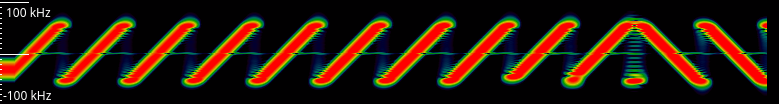
\includegraphics[width=0.95\textwidth]{images/LoRaFrame.png}
  \end{center}
  \caption{Example of capture needed for the machine learning algorithm}\label{fig:lorapreambule}
\end{figure}


After making the time synchronisation method work and discussing with Aqeel about the resulting captures, a clear issue came to us :
the frames were not captured with the same gap of samples each time. 


\begin{figure}[H]
  \begin{center}
    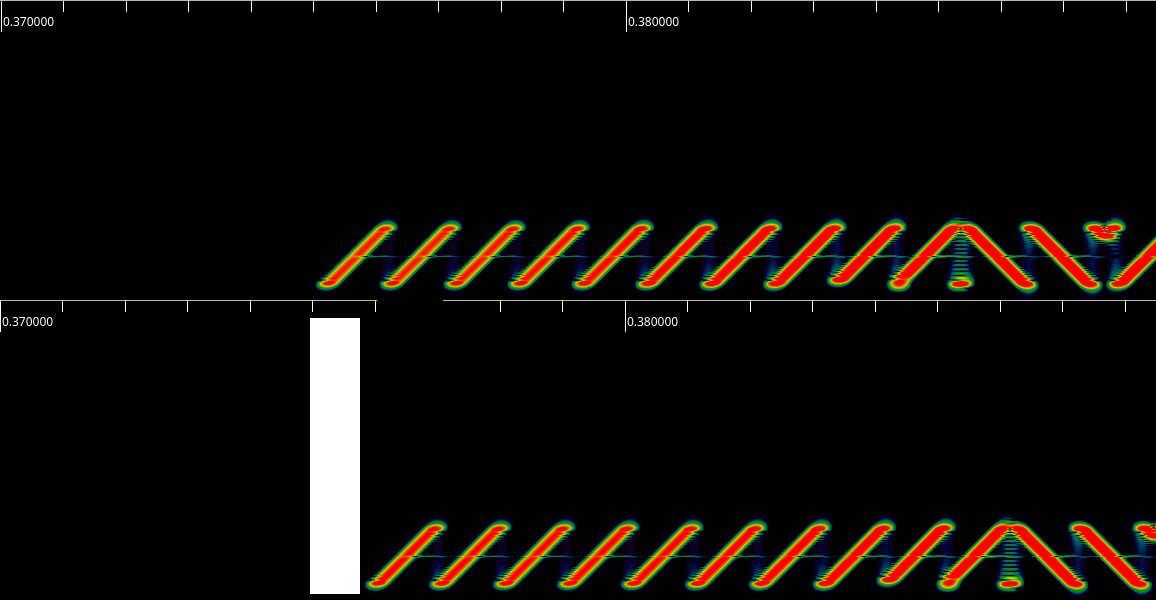
\includegraphics[width=0.95\textwidth]{images/gapDif.png}
  \end{center}
  \caption{Two captured LoRa preamble from the same device. Sample gap difference shown in white }\label{fig:GapDif}
\end{figure}

As shown in figure \ref{fig:GapDif}, in the captures made for a certain device, the start of the LoRa frame was not consistent. Due to this unconsistency, we wouldn't be able to post-process the captures correctly.

\newpage

\noindent
This was certainly due to random delays caused by :
\begin{enumerate}
  \item The transmitter waking up from its sleep to send the arduino a sendFlag
  \item The communication from the transmitter to arduino devices through Serial Ports
  \item The arduino device receiving the sendFlag and sending the lora frame
  \item The receiver switching from one device to another (implemented like a sleep)
\end{enumerate}

So, by itself, the time synchronisation method wouldn't be enough for the Captures to be usable even with postprocessing.

\subsection{LoRa detection}
There were two issues with the last LoRa detection implementation:
\begin{enumerate}
  \item The use of resampling before and after the detection 
  \item The gap in the beginning of captures 
\end{enumerate}
We decided to work on those issues to be able to have precise LoRa preamble captures for each frame.  

\section{Solutions found}
\subsection{Captures with time synchronisation method}
We decided to use detection in addition to time synchronisation.
So the file saver block would save only the detected LoRa preamble and not the whole period.

\subsection{LoRa detection}
With the help of its creator, we managed to remove the hardcoded sample rate and pass it as a parameter.

An example of the last year's capture saving flowgraph can be found at the figure \ref{fig:lastGRC}.\\
Compared to it at the figure \ref{fig:nowGRC} is the current capture saving flowgraph which doesn't need resampling.
\begin{figure}[H]
  \begin{center}
    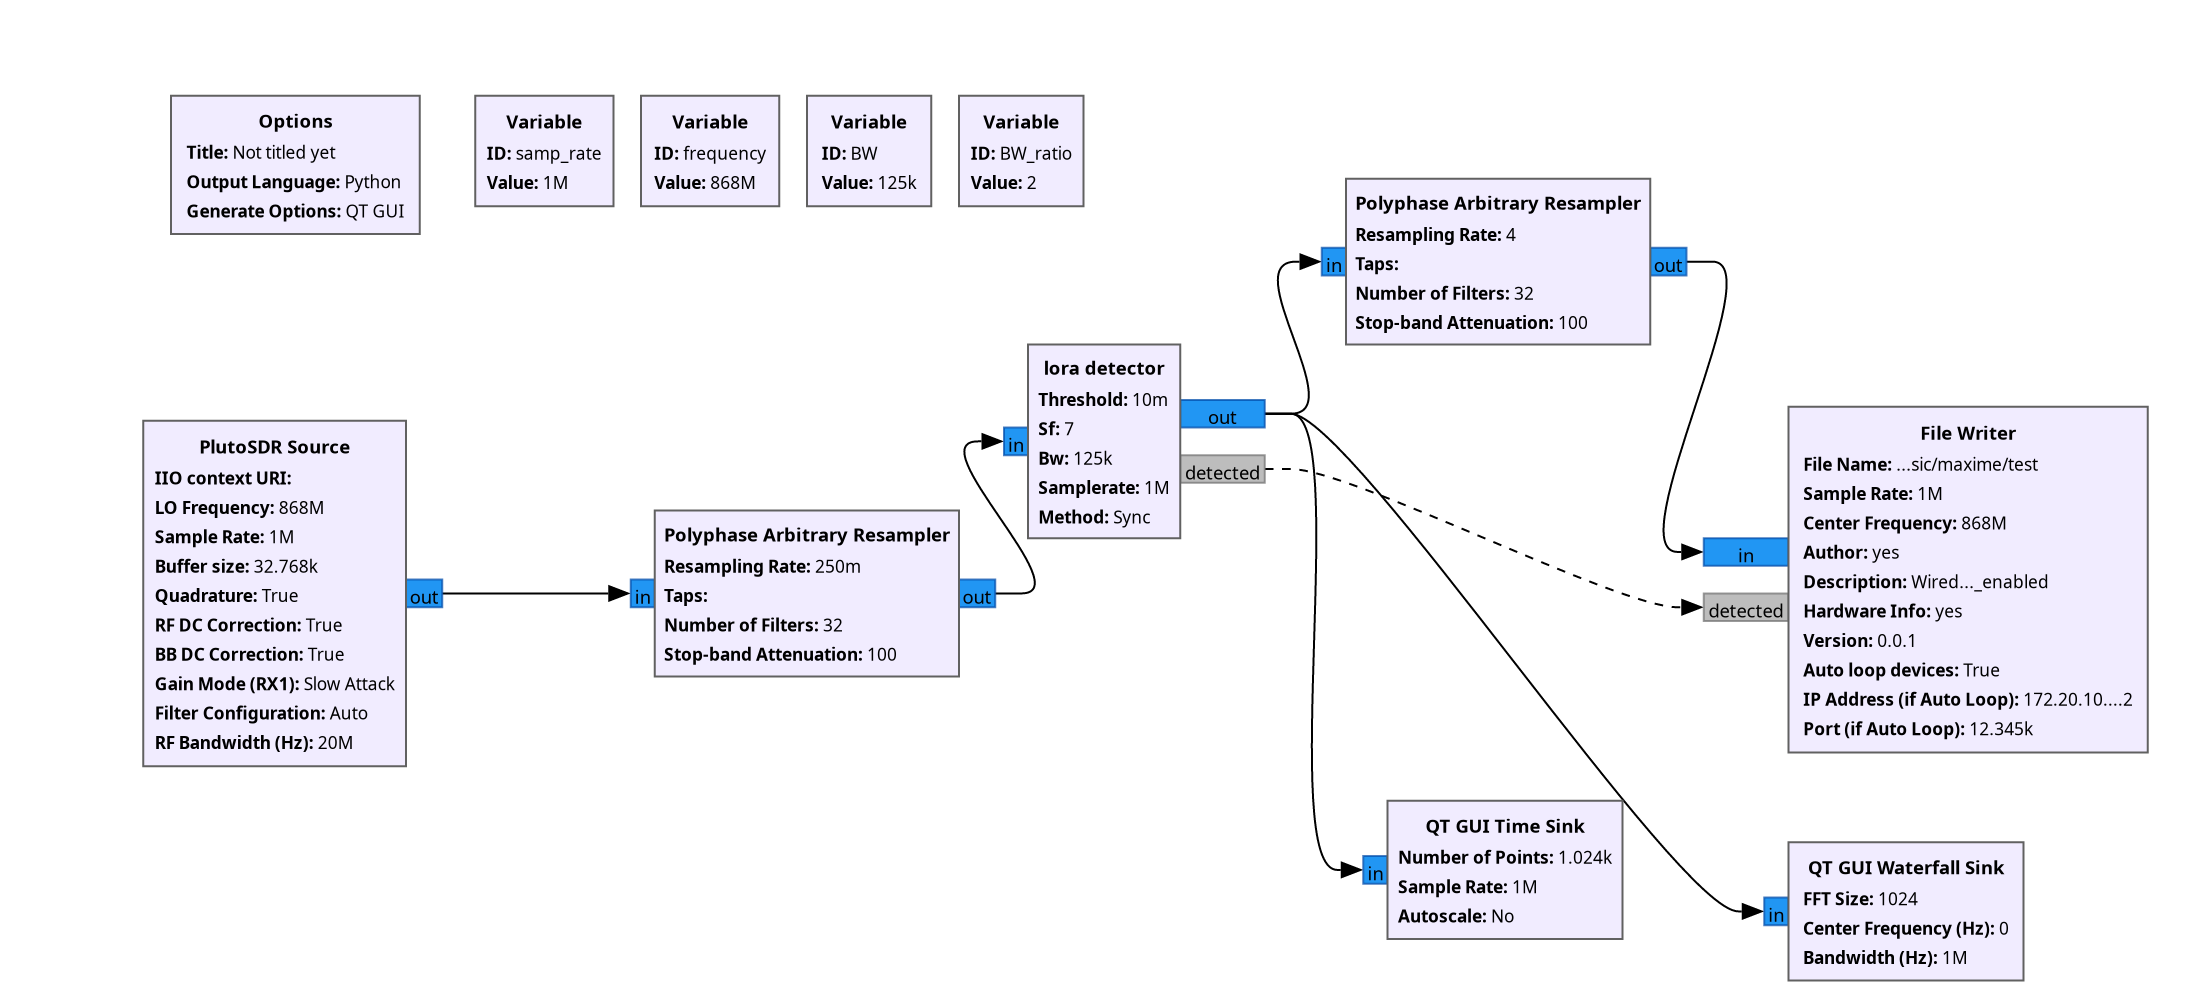
\includegraphics[width=0.95\textwidth]{images/lastGRCDetec.png}
  \end{center}
  \caption{Last year's capture flowgraph}\label{fig:lastGRC}
\end{figure}

\begin{figure}[H]
  \begin{center}
    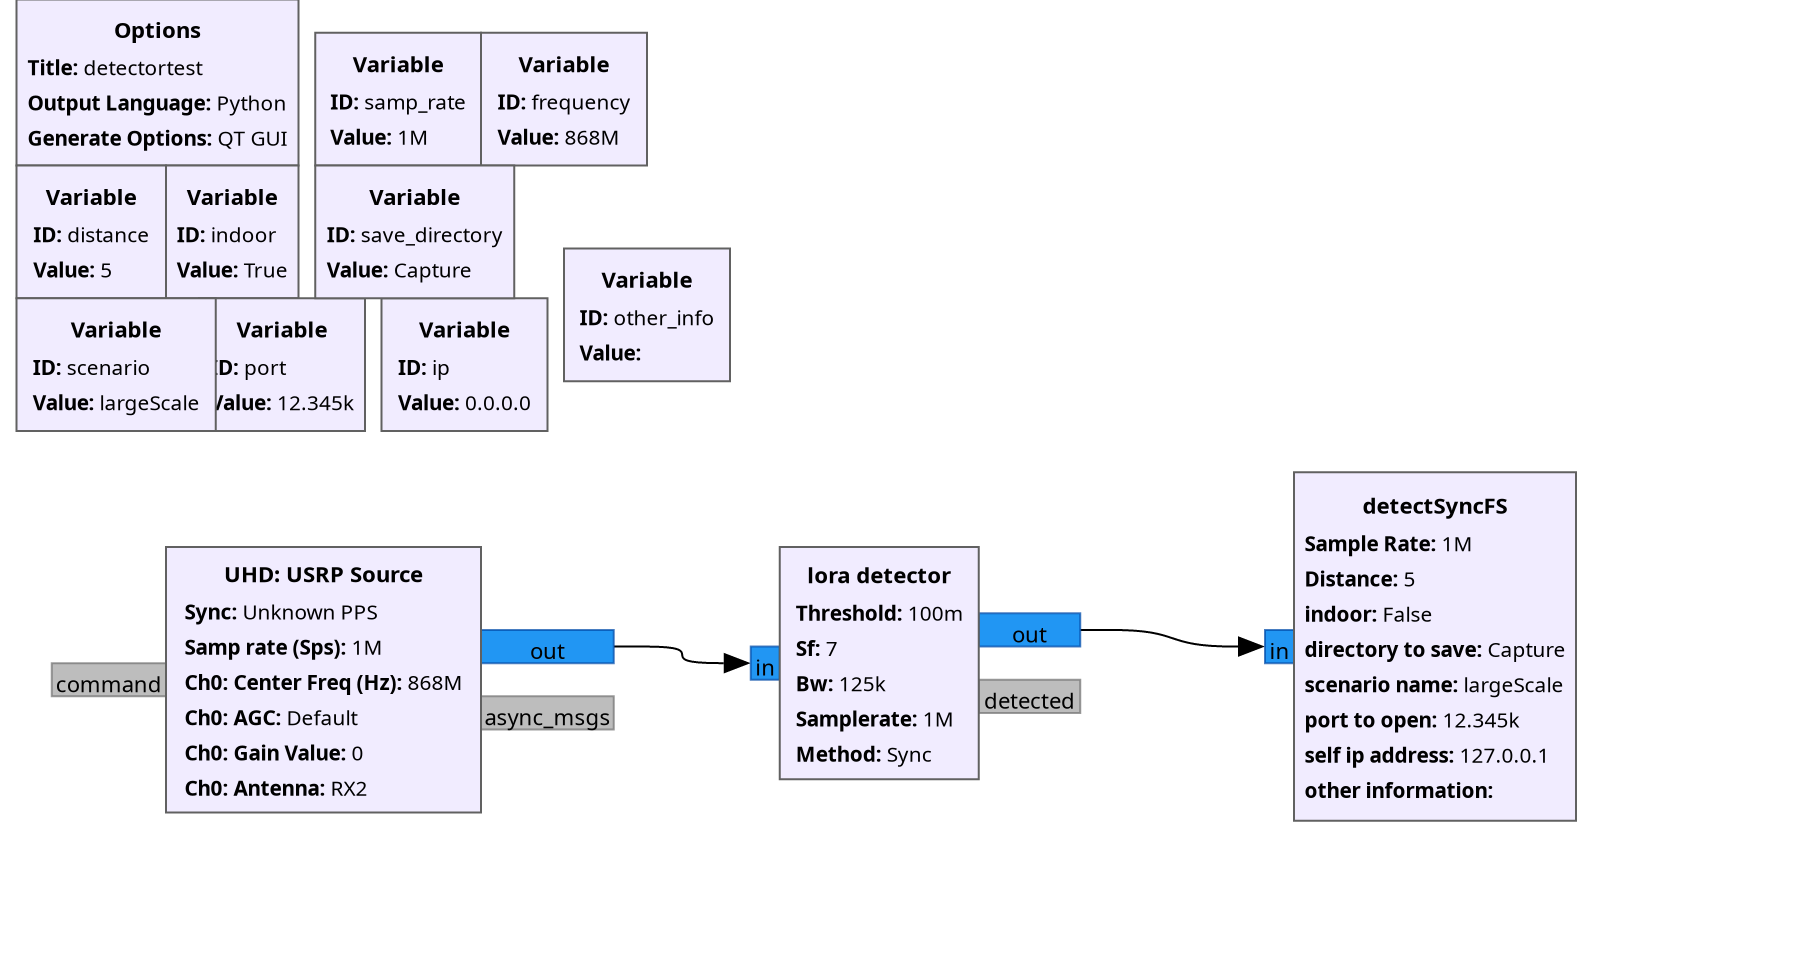
\includegraphics[width=0.95\textwidth]{images/nowGRCDetec.png}
  \end{center}
  \caption{Current capture flowgraph}\label{fig:nowGRC}
\end{figure}

\section{Summary}
By changing the LoRa preamble detector, I've managed to implement a working detection + synchronisation method for capturing and classifying the received LoRa frames.

In addition, I made this detection + synchronisation method robust by adding real time socket communication in case of a falling device. 

We found out that 2mm wide colson necklace were perfect for stabilizing the devices on the frame we will be using in large scale scenarios.


\section{Detection + time synchronisation implementation} \label{TSi}
There is basically 3 parts to this implementation: 
\begin{itemize}
  \item The receiver side capturing the LoRa frames
  \item The transmitter side in charge of controlling which device should transmit
  \item The Arduino implementation handling the transmission
\end{itemize}

The transmitter is in charge of taking all the transmission parameters such as frequency, bandwidth, spreading factor, number of frames to transmit per devices (cycles) and synchronisation parameters such as phase and period.

The receiver is in charge of capturing the LoRa frames and classify them by device.

The arduino devices transmit LoRa frames when the transmitter tells them to.

\vspace{1cm}

\subsection{Transmitter-arduino relation}
Let's first take a look at the relation between the transmitter and the arduino devices :

the first job of the transmitter is to communicate all the transmission parameters to all the arduino devices connected to it by sending an InitFlag followed by the parameters. 

Then when an arduino is initiated, it waits for a SendFlag for it to transmit a single LoRa frame. After Sending it, the arduino goes back to waiting for a SendFlag until it sent all the frames it had to.

A state machine showing this relation can be found in the figure \ref{ardSM}.

\begin{figure}[H]
  \begin{center}
    \includegraphics[width=0.7\textwidth]{images/arduinoStateMachine.jpg}
  \end{center}
  \caption{arduino state machine}\label{ardSM}
\end{figure}

In the WaitingForInitFlag state, the arduino's builtin LED blinks every seconds.\\
In the WaitingForSendFlag state, the arduino's builtin LED doesn't blink.\\
During the transmission of a LoRa frame, the arduino's builtin LED is lit up.

The behavior of the builtin LED then permits us to know in which state the arduino is at any time.


\subsection{Transmitter-receiver relation}
First, the receiver sets itself as a socket server on a certain port. The transmitter connects to this socket using the port and the receiver's IP address. Then, when the connection is done, the transmitter sends all the synchronisation parameters to the receiver such as : 
\begin{itemize}
  \item the starting time of transmission 
  \item a list of the devices ordered by device id
  \item the period between each transmission
\end{itemize}

Then, after the starting time is reached :\\
The transmitter sends a LoRa frame from the first device in the list and cycles the device's transmission each period.\\
The receiver waits for a detected LoRa frame to come from the LoRa detector and cycles the device's identifiers each period.

\subsection{cycling devices and frame classification}
For the receiver to rightfully classify the detected LoRa frames per device and frame count, I implemented a separate thread in charge of cycling those identifiers.

I had to thread it because the work function of the file saver wasn't running continuously, it only ran when there were incoming signals (so when LoRa frames were detected).

\subsection{Saving structure}
A saving directory and scenario name have to be given. 
The structure can be seen in figure \ref{savestruct}

\begin{figure}[H]
  \begin{center}
    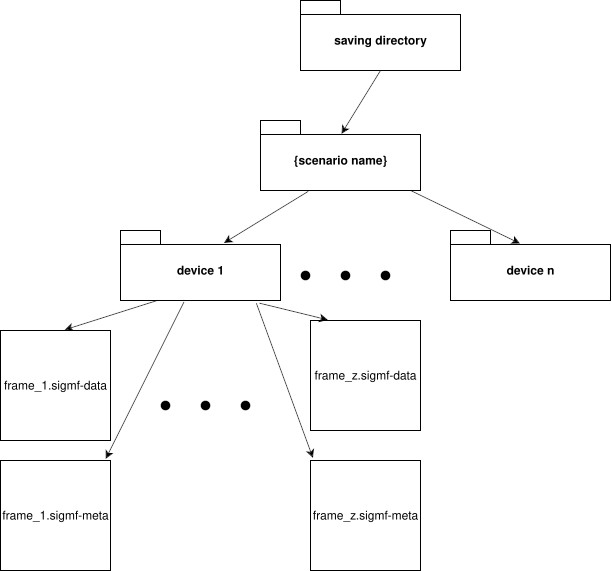
\includegraphics[width=0.6\textwidth]{images/save.jpg}
  \end{center}
  \caption{saving structure}\label{savestruct}
\end{figure}

Each .sigmf-meta files contains :
\begin{itemize}
  \item the data type (c32\_le)
  \item the frequency
  \item the sample rate
  \item the capture time
  \item a description taking the distance, outdoor/indoor and other possible parameters
\end{itemize}


\subsection{Arduino crash handling}
If at any point, a device is unreachable from the transmitter, the goal is to remove it from sending and receiving device lists. This will have the effect of it being ignored completely gaining the time it would have been taking.

When a device is detected as unreachable, a "remove" message is sent by the transmitter to the receiver followed by the device id to be removed, the restart time (for synchronisation purpose) and the device id to restart the reception/transmission on.

This permits us to remove any crashing device on both the receiver and transmitter.

To implement this method, the TCP connection between the receiver and transmitter had to be threaded to be able to react in real time.

\subsection{Improvements}
Some improvements can be made in this implementation :
\begin{itemize}
  \item use implicit header for the LoRa frame
  \item thread the file saving (it takes a lot of time and may be a treshold for minimum transmission period)
\end{itemize}

\section{Conclusion}
After testing on a larger scale (10 devices), the implementation works even with crashing devices.
The goal for the last two weeks of this Internship is to be able to capture and classify 15 devices in different scenarios. 
Some improvements can be made to make those captures faster.
% \printbibliography

\end{document}
